
The majority of our initial meetings consisted of creating a rough outline of how we envisioned our language. Much of the concept for the language was decided upon by Sankalpa, who was originally the one who suggested designing a quantum computing language. This strong foundation is what allowed us to create qlang.
 
\section{Project Management}
\subsection{ Planning}
Throughout the semester we met regularly to keep everyone up to date on the overall progress of the project. Initially, it was twice a week after class for short meetings, but as the semester went on, we began to meet nearly everyday. At the end of every week, there was a short session reviewing what was accomplished that week, as well as our goals for the upcoming week.

\subsection{Specification}
Upon creation, the LRM was the manifestation of our vision. However, it was almost immediately upon submitting the LRM that we realized that there were some changes that had to be made. This was a common theme throughout the development process. Even though we had a set ideal of what we wanted, the specification of the implementation varied during the course of our work. However, constantly thinking about how certain things would affect, or be influenced by, the LRM caused us to think more critically about our code. Though our LRM changed during the project lifetime, QLang evolved as well.

\subsection{Development}
To ensure the group as a whole was able to coordinate their independent work, we used Git as a distributed version control system. Each team member worked on an individual feature. When they were satisfied that their section was working and had passed unit tests, it was pushed into the master branch. Once it was pushed, the other team members looked over the feature and made suggestions as well as pointed out any bugs that were missed. This iterative process was repeated the entire project. 

\subsection{Testing}
We continuously performed unit tests throughout the development process. However, it was not until the end that we completed more rigorous acceptance testing. This was due to the continued evolution of our language as well as features. One constant throughout the project was a configurable test script that allowed us to complete the compilation process to a certain point. This allowed us to isolate tests for the individual parts of the compiler such as the AST or code generator.

\section{Style Guide}
The following coding guidelines were generally followed while coding:

\begin{itemize}
	\item One statement per a line
	\item Each block of code following a “let” statement is indented
	\item Helper functions are written for commonly reused code
\end{itemize}
	
\section{Project Timeline}
Commits to master, excluding merge commits
\begin{figure}[h]
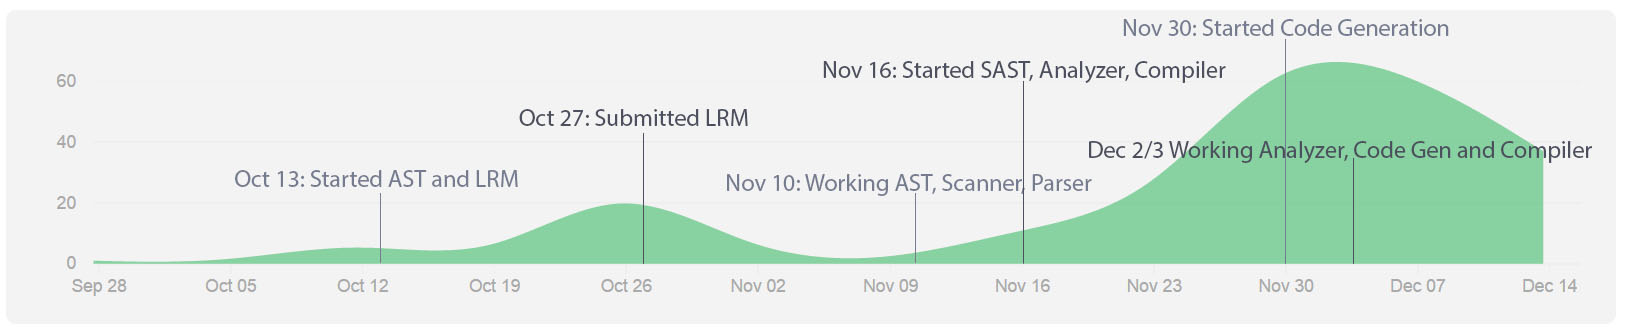
\includegraphics[width=16cm]{teamCommitGraph}
\centering
\end{figure}\\
The above graph shows the project timeline for the QLang compiler. It represents the number of commits over the course of the project, with a total of 397 commits. Work was generally centered around large project deadlines but slowing down near the end of the project as we were wrapping up.

\section{Roles and Responsibilities}
Christopher Campbell  - System Architect (coded the greater part of the semantics)\\
Sankalpa Khadka - Language Guru (designed the majority of the features of our language)\\
Winnie Narang – Testing Verification and Validation (created the bulk of the test suite)\\
Jonathan Wong – Manager (built the QLang C++ library)\\
C\'ement Canonne - LaTex

\section{Software Development Environment}

The QLang project was built on a combination of OS X and Arch Linux platforms. As stated above, Git was used as a distributed version control system. The compiler itself was written using both vim and sublime. The project was done mostly in OCaml, but a QLang C++ library was created to augment the C++ Matrix library Eigen that is used for much of the linear algebra. Since our code was compiled to C++, g++ was used to compile the code into an executable. Lastly, Bash/shell scripts and makefiles were used to automate compilation and testing.

\section{Project Log}
Below is an excerpt from our git log in the format of “<YYYY-MM-DD>: <Author> - <Commit Message>”.

\begingroup
    \fontsize{9pt}{10pt}\selectfont
	\verbatiminput{projectLog.txt} 
\endgroup



